% Created 2020-03-20 vie 16:05
% Intended LaTeX compiler: pdflatex
\documentclass[presentation,aspectratio=1610]{beamer}
\usepackage[utf8]{inputenc}
\usepackage[T1]{fontenc}
\usepackage{graphicx}
\usepackage{grffile}
\usepackage{longtable}
\usepackage{wrapfig}
\usepackage{rotating}
\usepackage[normalem]{ulem}
\usepackage{amsmath}
\usepackage{textcomp}
\usepackage{amssymb}
\usepackage{capt-of}
\usepackage{hyperref}
\usepackage{khpreamble}
\usepackage{pgfplots}
\usepackage{pdfpages}
\usepgfplotslibrary{groupplots}
\usetheme{default}
\author{Kjartan Halvorsen}
\date{\today}
\title{Pneumatic tank system}
\hypersetup{
 pdfauthor={Kjartan Halvorsen},
 pdftitle={Pneumatic tank system},
 pdfkeywords={},
 pdfsubject={},
 pdfcreator={Emacs 26.3 (Org mode 9.3.6)}, 
 pdflang={English}}
\begin{document}

\maketitle

\section{Intro}
\label{sec:org8bfd10f}
\begin{frame}[label={sec:org5f5b8a7}]{Lab experiment}
\begin{center}
\includegraphics[width=\linewidth]{../../figures/tank-lab-setup.png}
\end{center}
\end{frame}

\begin{frame}[label={sec:orgadadc1a}]{Simulink simulation}
\begin{center}
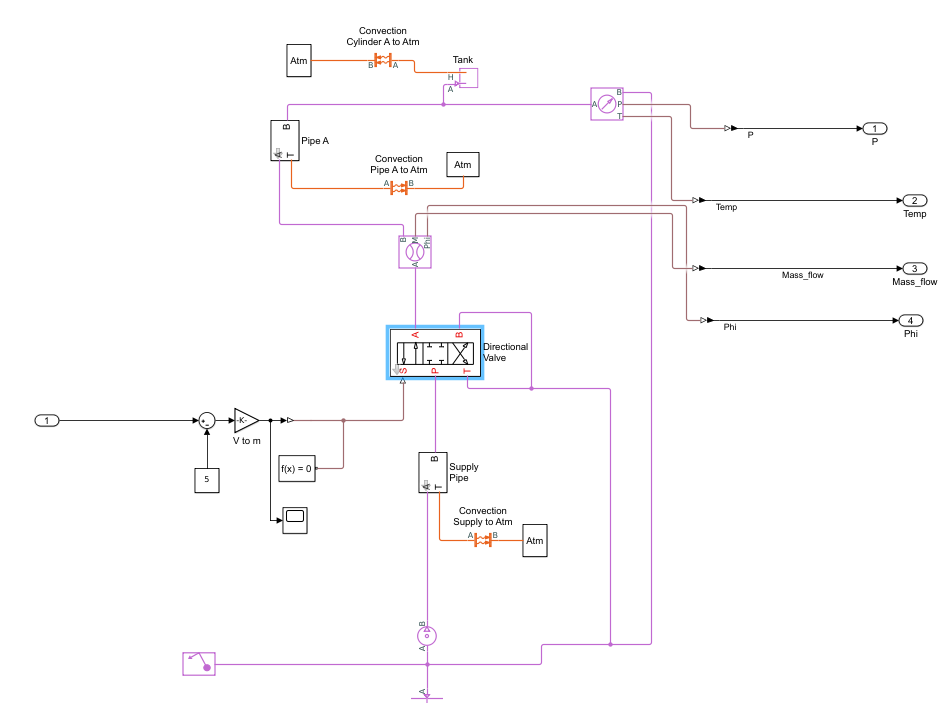
\includegraphics[width=0.8\linewidth]{../../figures/tank-simscape-model.png}
\end{center}
\end{frame}

\section{Modeling}
\label{sec:orgfdff3e1}
\begin{frame}[label={sec:org8513ecf}]{Pneumatic elements}
\begin{center}
\includegraphics[width=\linewidth]{../../figures/tank-lab-setup.png}
\end{center}
\end{frame}

\begin{frame}[label={sec:org19a4887}]{Valve}
\begin{center}
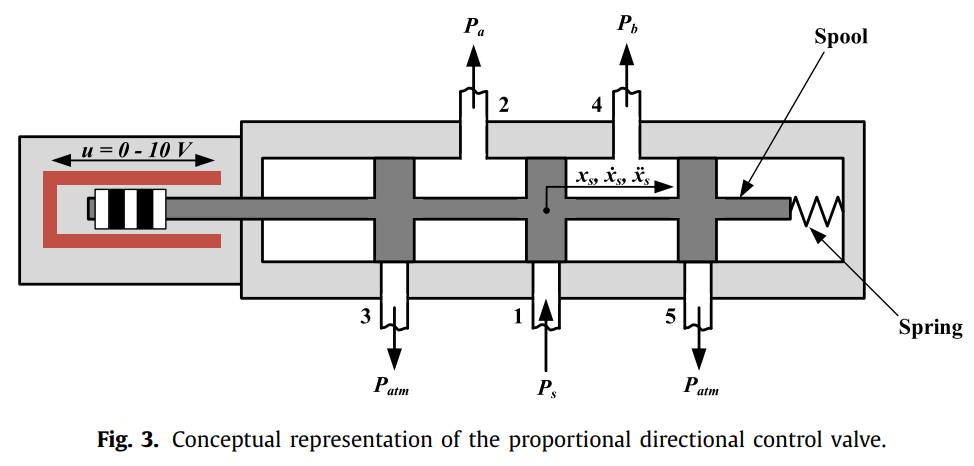
\includegraphics[width=\linewidth]{../../figures/proportional-directional-control-valve-concept.png}
\end{center}
\begin{LATEX}
  \tiny From ''An improved nonlinear modelling and identification
methodology of a servo-pneumatic actuating system with
complex internal design for high-accuracy motion control
applications'' Simulation Modelling Practice and Theory 2017
\end{LATEX}
\end{frame}

\begin{frame}[label={sec:org1059008}]{Valve, contd}
\begin{center}
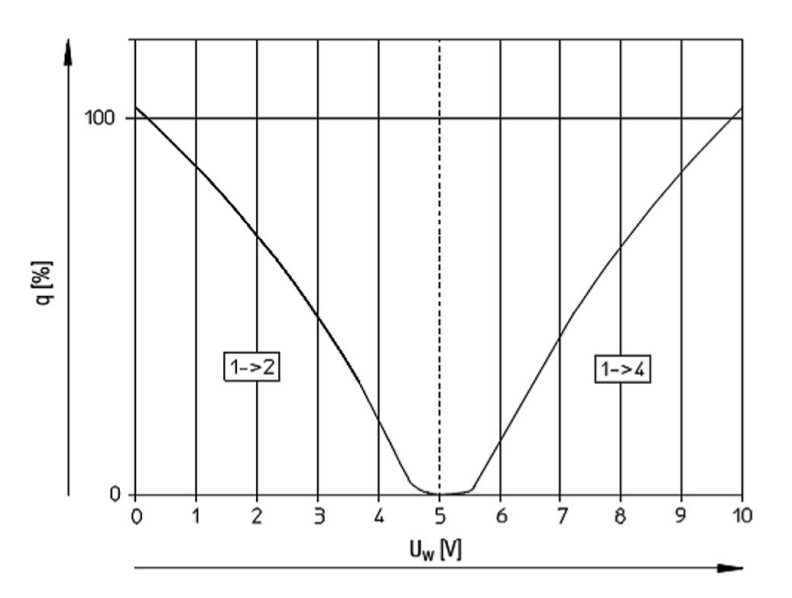
\includegraphics[width=0.7\linewidth]{../../figures/valve-volt-opening.png}
\end{center}
\end{frame}

\begin{frame}[label={sec:org402cb77}]{Experiment}
\begin{center}
\includegraphics[width=0.65\linewidth]{../../figures/tank-lab-setup.png}
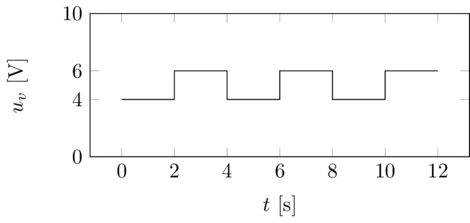
\includegraphics[width=0.35\linewidth]{../../figures/square-wave-pressure-valve.png}
\end{center}
\end{frame}

\begin{frame}[label={sec:org382e73f}]{Result}
\begin{center}
\includegraphics[width=0.7\linewidth]{../../figures/tank-response-scope.png}
\end{center}
\end{frame}

\begin{frame}[label={sec:orgdb8f573}]{Simscape}
\begin{center}
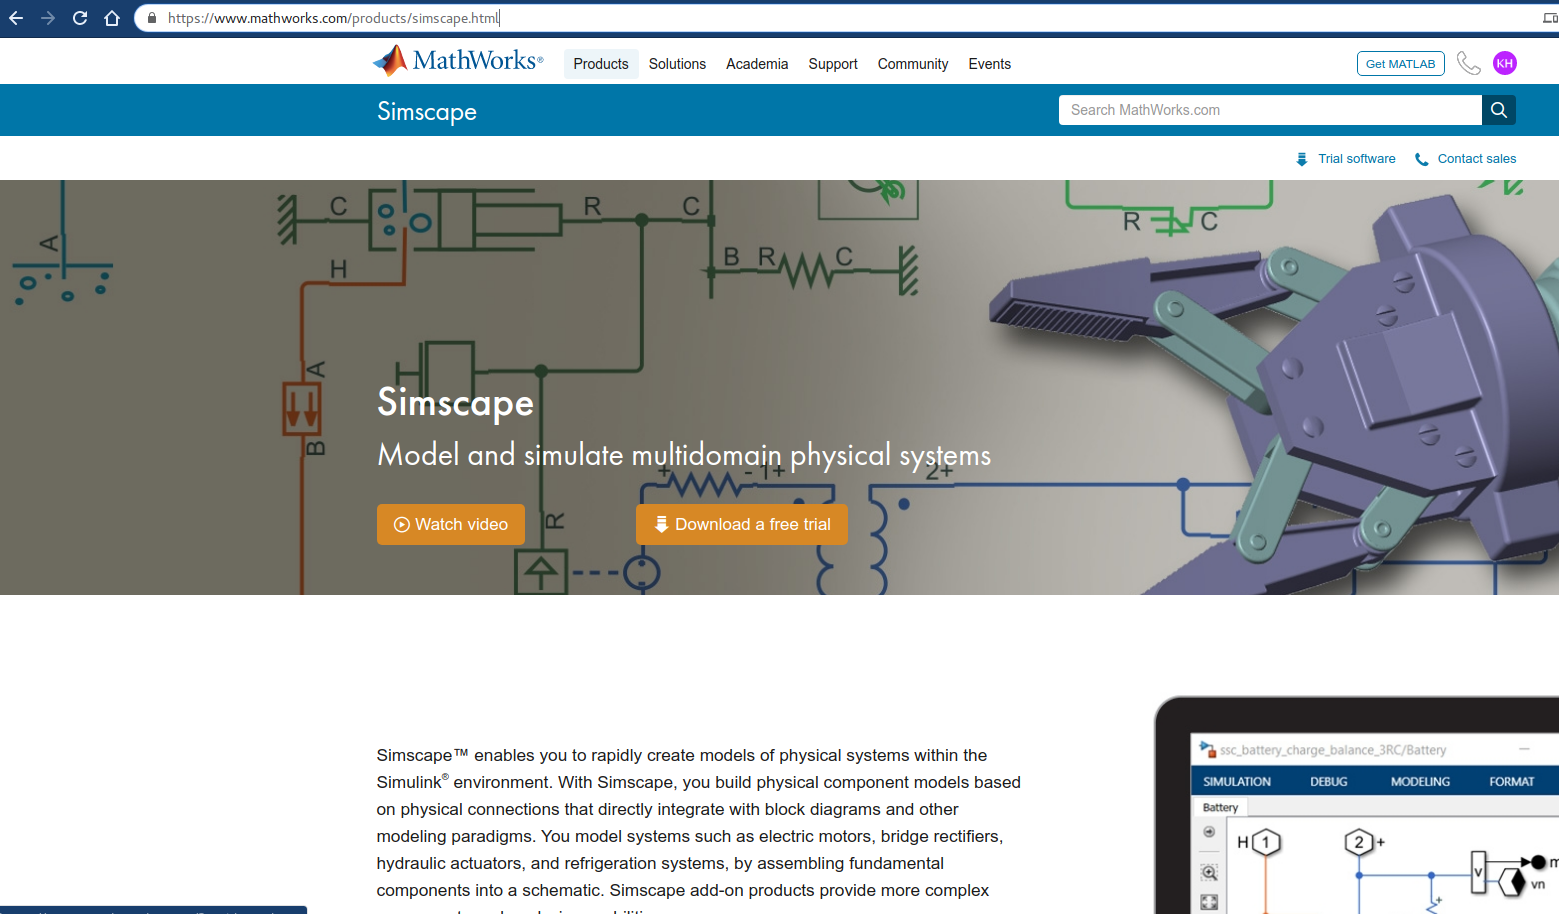
\includegraphics[width=\linewidth]{../../figures/simscape.png}
\end{center}
\end{frame}

\begin{frame}[label={sec:org2b5a140}]{Simulation model}
\begin{center}
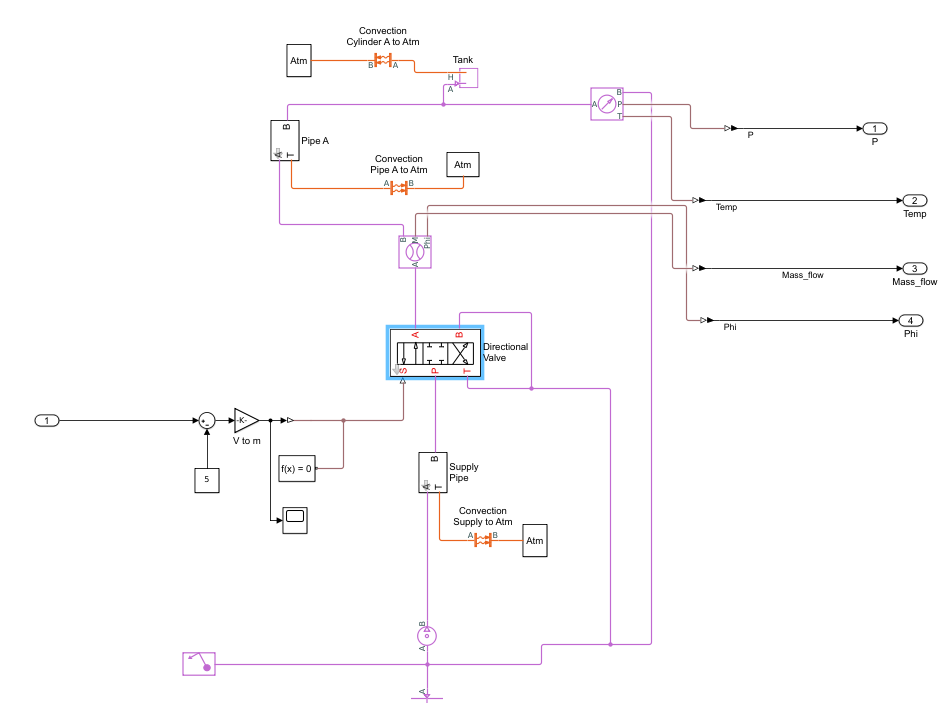
\includegraphics[width=0.8\linewidth]{../../figures/tank-simscape-model.png}
\end{center}
\end{frame}
\end{document}